\documentclass[a4paper]{article}

\usepackage[T2A]{fontenc}
\usepackage[utf8]{inputenc}
\usepackage[russian]{babel}


\usepackage{graphicx}
\usepackage{float}
\usepackage{mathtools}
\usepackage{wrapfig}
\usepackage{amsfonts, amssymb, amsmath, latexsym}
\usepackage{nicefrac}
\usepackage{hhline}
\usepackage{multirow}
\usepackage[colorinlistoftodos,bordercolor=orange,backgroundcolor=orange!20,linecolor=orange,textsize=scriptsize]{todonotes}
\usepackage[colorlinks=true,linkcolor=blue,citecolor=blue]{hyperref}       % hyperlinks
\usepackage{nicefrac}       % compact symbols for 1/2, etc.
\usepackage{nameref}
\usepackage{booktabs}       % professional-quality tables

\usepackage{algorithm}
\usepackage{algpseudocode}

\usepackage{xcolor, colortbl}
\usepackage{etoolbox}

% \graphicspath{ {./} }

\usepackage[verbose=true,letterpaper]{geometry}

\newgeometry{
    textheight=9in,
    textwidth=5.5in,
    top=1in,
    headheight=12pt,
    headsep=25pt,
    footskip=30pt
}

\usepackage{epigraph}

%

\newcommand{\argmin}{\mathop{\arg\!\min}}
\newcommand{\argmax}{\mathop{\arg\!\max}}

\newcommand{\Var}{\mathbb{V}}
\newcommand{\Exp}{\mathbb{E}}
\newcommand{\Cov}{\text{Cov}}
\newcommand{\makebold}[1]{\boldsymbol{#1}}
\newcommand{\mean}[1]{\overline{#1}}
\newcommand{\eps}{\varepsilon}
\renewcommand{\epsilon}{\varepsilon}

\newcommand{\partfrac}[2]{\frac{\partial #1}{\partial #2}}
\newcommand{\ttt}[1]{\texttt{#1}}
\newcommand{\term}[1]{\textbf{#1}}

\newcommand{\la}{\langle}
\newcommand{\ra}{\rangle}

\newcommand{\lp}{\left(}
\newcommand{\rp}{\right)}
\newcommand{\lf}{\left\{}
\newcommand{\rf}{\right\}}
\newcommand{\ls}{\left[}
\newcommand{\rs}{\right]}
\newcommand{\lv}{\left|}
\newcommand{\rv}{\right|}

\newcommand*{\affaddr}[1]{#1} % No op here. Customize it for different styles.
\newcommand*{\affmark}[1][*]{\textsuperscript{#1}}


\usepackage{amsthm}

\theoremstyle{definition}
\newtheorem{definition}{Определение}[section]

\newtheorem{exercise}{Задача}[section]

\newtheorem*{solution}{Решение}
\theoremstyle{remark}
\newtheorem*{remark}{Remark}

\makeatletter
\renewcommand{\l@section}{\@dottedtocline{1}{0em}{2.1em}}
\makeatother

% \setlength\epigraphwidth{.8\textwidth}
\setlength\epigraphrule{0pt}

\title{Работа 4.8 А \\ Резонанс токов}
\author{Шарапов Денис, Зелёный Николай, Б05-005}
\date{}

\usepackage{fancyhdr}
\pagestyle{fancy}
\fancyhf{}
\rhead{Работа 4.8 А}
\lhead{}
\cfoot{\thepage}
\usepackage{subcaption}
\usepackage[font={small}]{caption}

\begin{document}

    \maketitle
    \tableofcontents
    \newpage
    
\section{Аннотация}

\textbf{Цель работы:} изучение параллельной цепи переменного тока, наблюдение резонанса токов. \medskip
 
\noindent \textbf{В работе используются:} лабораторный трансформатор (ЛАТР), разделительный понижающий трансформатор, ёмкость, дроссель с переменной индуктивностью, три амперметра, вольтметр, реостат, электронный осциллограф, омметр, мост переменного тока.
 
\section{Теоретические сведения}

В работе изучается параллельный контур, одна из ветвей которого содержит индуктивность $L$, другая --- ёмкость $C$. Через $r_L$ обозначено активное сопротивление катушки, которое включает в себя как чисто омическое сопротивление катушки, так и сопротивление, связанное с потерями энергии при перемагничивании сердечника катушки. Активным сопротивлением ёмкостной ветви контура можно пренебречь, т. к. используемый в работе конденсатор обладает малыми потерями.

\subsection*{Экспериментальная установка}

Схема экспериментальной установки приведена на рисунке 1. Напряжение от сети (220~В, 50 Гц) с помощью ЛАТР-а через понижающий трансформатор Тр подаётся на параллельный контур, содержащий конденсатор ($C = 120$ мкФ) и катушку, индуктивность которой зависит от глубины погружения сердечника. Полный ток в цепи измеряется с помощью многопредельного амперметра $A_1$; для измерения токов в $L$- и $C$-ветвях используются два одинаковых амперметра $A_2$ и $A_3$; напряжение на контуре контролируется электронным вольтметром $V$. Последовательно с контуром включён резистор~$r$~--- реостат с полным сопротивлением $\approx 100$ Ом.

\begin{figure}[h!]
    \centering
    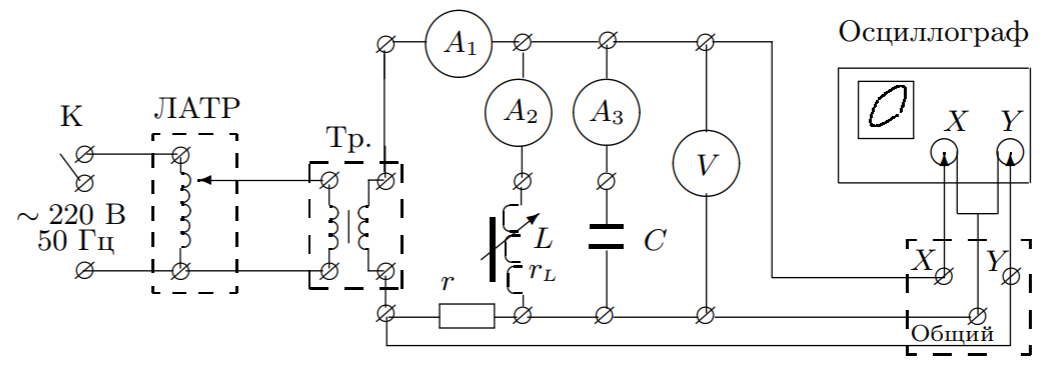
\includegraphics[width = 325pt]{image/picture1.png}
    \caption{Схема для исследования резонанса токов}
\end{figure}

Для наблюдения за сдвигом фаз между полным током и напряжением на контуре используется осциллограф. Сигнал, пропорциональный току, снимается с резистора $r$ и подаётся на вход $Y$ осциллографа. На вход $X$ подаётся напряжение непосредственно с контура. При наличии сдвига
фаз между этими напряжениями на экране виден эллипс, а при нулевом сдвиге фаз эллипс вырождается в прямую.
\medskip

В работе предлагается снять при постоянном напряжении $U$ зависимости токов $I_L$, $I_C$ и полного тока $I$ от индуктивности катушки (глубины погружения сердечника), а также определить резонансные характеристики контура: полное сопротивление $R_{\text{рез}}$, добротность $Q$, активное сопротивление $r_L$ и индуктивность катушки $L_{\text{рез}}$.

\section{Ход работы}

\begin{enumerate}
    \item Снимем зависимости $I$, $I_L$, $I_C$ от координаты сердечника при $U = const$.
    \item Измерим резонансные значения трёх токов.
    \item Измерим сопротивление витков катушки с помощью омметра.
    \item Измерим активное сопротивление катушки $r_L$ и резонансное значение индуктивности $L$ с помощью моста.
\end{enumerate}

\section{Результаты измерений и обработка данных}

\subsection{Зависимости токов от положения сердечника}

Поддерживая $U = const$, найдём зависимости токов $I$, $I_L$, $I_C$ от координаты сердечника~$x$. Результаты измерений представлены в таблице 1:

\begin{table}[h!]
    \centering
    \caption{Результаты измерений зависимости токов от координаты}
    \begin{tabular}{|c|c|c|c|}
    \hline
    \rowcolor[HTML]{FFFFFF}
    \textbf{$x$, мм} & \textbf{$I$, мА} & \textbf{$I_L$, мА} & \textbf{$I_C$, мА} \\ \hline
    10 & 270 & 0 & 330 \\ \hline
    12 & 245 & 50 & 320 \\ \hline
    15 & 210 & 80 & 310 \\ \hline
    20 & 185 & 90 & 310 \\ \hline
    25 & 160 & 100 & 310 \\ \hline
    30 & 140 & 120 & 300 \\ \hline
    35 & 130 & 180 & 310 \\ \hline
    40 & 110 & 200 & 300 \\ \hline
    45 & 90 & 210 & 310 \\ \hline
    50 & 70 & 230 & 310 \\ \hline
    55 & 50 & 250 & 310 \\ \hline
    60 & 25 & 270 & 300 \\ \hline
    65 & 10 & 300 & 310 \\ \hline
    67 & 10 & 320 & 320 \\ \hline
    \end{tabular}
    \end{table}

По таблице 1 построим график зависимости токов от координаты:

\begin{figure}[h!]
    \centering
    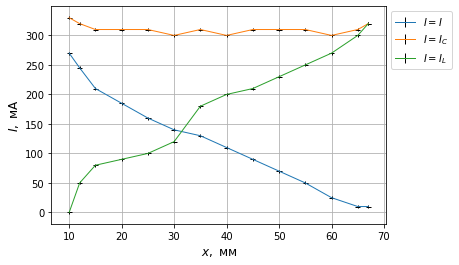
\includegraphics[width = 280pt]{image/graph1.png}
    \caption{График зависимости токов от положения сердечника}
\end{figure}

\subsection{Расчёт величин}

\noindent Рассчитаем добротность контура через токи:

$$Q = \frac{I_C^{\text{рез}}}{I^{\text{рез}}} = \frac{I_L^{\text{рез}}}{I^{\text{рез}}} = 32,00 \pm 0,25,$$ где $I_{\text{рез}} \approx 10$ мА, $I_C^{\text{рез}} = 320$ мА, $I_L^{\text{рез}} = 320$ мА. \medskip

\noindent Рассчитаем резонансное сопротивление через полный ток и напряжение: $$R^{\text{рез}} = \frac{U}{I^{\text{рез}}} \approx (1,00 \pm 0,01) \;\text{кОм},$$ где $U = 10$ В. \medskip


\noindent Рассчитаем индуктивность $L^{\text{рез}}$: $$L^{\text{рез}} = \frac{1}{Q\omega_0^2} \approx (8,5 \pm 0,8)\cdot 10^{-2} \;\text{Гн},$$ где $\omega_0 = 2\pi\nu$, $\nu = 50$ Гц. \medskip

\noindent Рассчитаем сопротивление $r_L$: $$r_L = \frac{1}{Q\omega_0 C} \approx 8,3 \pm 0,8 \;\text{Ом}.$$ \medskip

\noindent Рассчитаем индуктивность $L$: $$L = \frac{U}{\omega_0 I^{\text{рез}}_L} \approx (10,0 \pm 0,9) \cdot 10^{-2} \;\text{Гн}.$$

\subsection{Векторная диаграмма}

Построим векторную диаграмму (масштаб нарушен в силу большого отличия модуля векторов; угол между векторами $\mathbf{I}^{\text{рез}}$ и $\mathbf{U}_L^{\text{рез}}$ ненулевой):

\begin{figure}[h!]
    \centering
    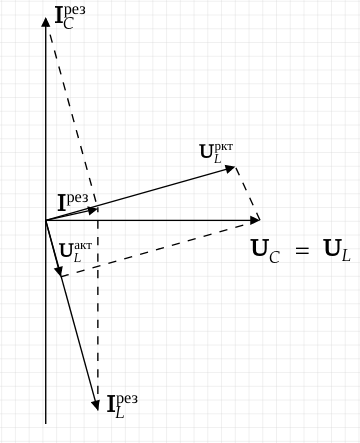
\includegraphics[width = 180pt]{image/picture2.png}
    \caption{Векторная диаграмма токов}
\end{figure}

C помощью векторной диаграммы рассчитаем значения величин $r_L$ и $L_{\text{рез}}$. Их результаты вместе со всеми измерениями работы занесём в таблицу 2.

\subsection{Результаты работы}

Результаты выполнения работы представлены в таблице 2.

\begin{table}[h!]
    \centering
    \caption{Результаты выполнения работы}
    \begin{tabular}{|c|c|c|c|c|c|}
    \hline
              & Омметр & Мост & $f(U^{\text{рез}}, I_L^{\text{рез}})$ & $f(Q)$ & Диаграмма \\ \hline
    $r_L$, Ом & $9,9$    & $8,8$  & ---       & $8,3 \pm 0,8$ & $3,0 \pm 0,9$       \\ \hline
    $L$, мГн  & ---    & $65,2$ & $100,0 \pm 9,0$     & $85,0 \pm 8,0$ & $96,0 \pm 10,0$      \\ \hline
    \end{tabular}
    \end{table}

\section{Вывод}

В работе была изучена параллельная цепь переменного тока, был изучен резонанс токов. \medskip

\noindent В ходе работы:
\begin{enumerate}
    \item были изучены зависимости токов от координаты сердечника;
    \item были измерены резонансные значения трёх токов;
    \item были измерены индуктивность и сопротивление витков катушки тремя способами (таблица 2): с помощью моста и омметра; с помощью добротности системы; с помощью векторной диаграммы.
\end{enumerate}

\end{document}
